%---------- Inleiding ---------------------------------------------------------

% TODO: Is dit voorstel gebaseerd op een paper van Research Methods die je
% vorig jaar hebt ingediend? Heb je daarbij eventueel samengewerkt met een
% andere student?
% Zo ja, haal dan de tekst hieronder uit commentaar en pas aan.

%\paragraph{Opmerking}

% Dit voorstel is gebaseerd op het onderzoeksvoorstel dat werd geschreven in het
% kader van het vak Research Methods dat ik (vorig/dit) academiejaar heb
% uitgewerkt (met medesturent VOORNAAM NAAM als mede-auteur).
% 
\newcommand{\figref}[1]{(Zie \hyperref[#1]{figuur: \ref{#1}})}

\section{Inleiding}%
\label{sec:inleiding}

In de hedendaagse samenleving is er een groeiende behoefte aan technologieën die de communicatie tussen doven en horenden vergemakkelijken. Een van de meest veelbelovende ontwikkelingen op dit gebied is de real-time vertaling van Vlaamse Gebarentaal (VGT) naar tekst, waarbij gebruik wordt gemaakt van kunstmatige intelligentie (AI) en computer vision. VGT, de taal die door de Vlaamse dovengemeenschap wordt gebruikt, is een volwaardige taal die, net als andere gesproken talen zoals Nederlands en Frans, erkend wordt door de taalkundige gemeenschap. Het is belangrijk op te merken dat VGT, net als gesproken talen, regionale variaties kent, wat de complexiteit van de vertaling vergroot \autocite{vanmeerbergen2000simultane}.

De structuur van VGT is hiërarchisch, wat betekent dat elk gebaar kan variëren in betekenis afhankelijk van specifieke details, zoals handvorm, beweging en gezichtsuitdrukkingen. \autocite{469340}
Deze variabiliteit maakt het noodzakelijk om geavanceerde algoritmen te ontwikkelen die in staat zijn om deze nuances te herkennen en correct om te zetten naar tekst. 
Recent onderzoek heeft aangetoond dat AI-technologieën, zoals deep learning en convolutionele neurale netwerken (CNN), effectief kunnen worden ingezet voor gebarentaalherkenning.\autocite{10.52756/ijerr.2023.v34spl.004}\autocite{10.17485/ijst/v16i45.2583}
Door gebruik te maken van camera's op smartphones en andere apparaten kan een systeem worden ontwikkeld dat in real-time gebaren herkent en omzet in geschreven tekst.
Deze technologische vooruitgang belooft een aanzienlijke impact te hebben op de toegankelijkheid en inclusie van de dove gemeenschap, waardoor zij beter kunnen communiceren met de horende wereld. Dit document onderzoekt de huidige stand van zaken op het gebied van AI-gestuurde VGT-herkenning en de potentiële toepassingen en uitdagingen die gepaard gaan met de implementatie van dergelijke systemen.

\section{Literatuurstudie}%
\label{sec:literatuurstudie}

% Voor literatuurverwijzingen zijn er twee belangrijke commando's:
% \autocite{KEY} => (Auteur, jaartal) Gebruik dit als de naam van de auteur
%   geen onderdeel is van de zin.
% \textcite{KEY} => Auteur (jaartal)  Gebruik dit als de auteursnaam wel een
%   functie heeft in de zin (bv. ``Uit onderzoek door Doll & Hill (1954) bleek
%   ...'')

%---------- Methodologie ------------------------------------------------------
\section{Methodologie}%
\label{sec:methodologie}
\subsection{Fase 1: Data-acquisitie}
In de eerste en meest cruciale fase van het onderzoek zal de benodigde data worden verzameld.
Voor het verzamelen van de data zal gebruik worden gemaakt van verschillende bronnen.
Deze bronnen zullen bestaan uit bestaande datasets, zoals de VGT-dataset van de Universiteit van Gent.
Daarnaast zullen er ook nieuwe datasets worden gecreëerd door middel van het opnemen van VGT-gebaren met behulp van een camera.
Deze datasets zullen worden gebruikt om het model te trainen en te valideren.
Voor deze fase een periode van 2 weken duren. \figref{fig:gantt_tijd}
\subsection{Fase 2: Preprocessing}
Voor het Preprocessen van de data wordt er weer een werktijd van 2 weken voorzien.\figref{fig:gantt_tijd}
Hier zullen de datasets worden geanalyseerd en gezuiverd.
De datasets zullen samengevoegd worden tot één dataset en worden opgedeeld in een trainingsset en een testset.
Het zal ook alle data juist labelen als dit nog niet correct is gebeurd.
\subsection{Fase 3: Modeltraining}
In de derde fase van het onderzoek zal het model worden getraind.
Dit zal de meeste tijd innemen van het onderzoek, namelijk 4 weken. \figref{fig:gantt_tijd}
Er zal een deep learning model worden ontwikkeld dat in staat is om VGT-gebaren te herkennen en om te zetten in tekst.
Hier zullen ook meerdere modellen getest worden om te kijken welk model het beste presteert.
De modellen zullen gekozen worden aan de hand van de literatuurstudie.
De modellen trainen zelf zal 3 weken duren en de laatste week zal dienen om de modellen te testen en te vergelijken.\figref{fig:gantt_tijd}
\subsection{Fase 4: Real-time implementatie}
In de vierde fase van het onderzoek zal het getrainde model worden aangepast zodat het real-time zou kunnen werken.
Deze fase zal 4 weken duren.\figref{fig:gantt_tijd}
Hier zal prunning en quantization worden toegepast om het model te optimaliseren voor real-time gebruik.
\subsection{Fase 5: Evaluatie \& Validatie}
In de laatste fase van het onderzoek zal het model worden geëvalueerd en gevalideerd.
Deze fase zal 2 weken duren.\figref{fig:gantt_tijd}
Het model zal worden getest op een nieuwe dataset en de resultaten zullen worden geanalyseerd.
Moesten er nog enige fouten zijn in het model zullen deze worden aangepast en zal het model opnieuw worden getest.

\begin{figure}[h!]
  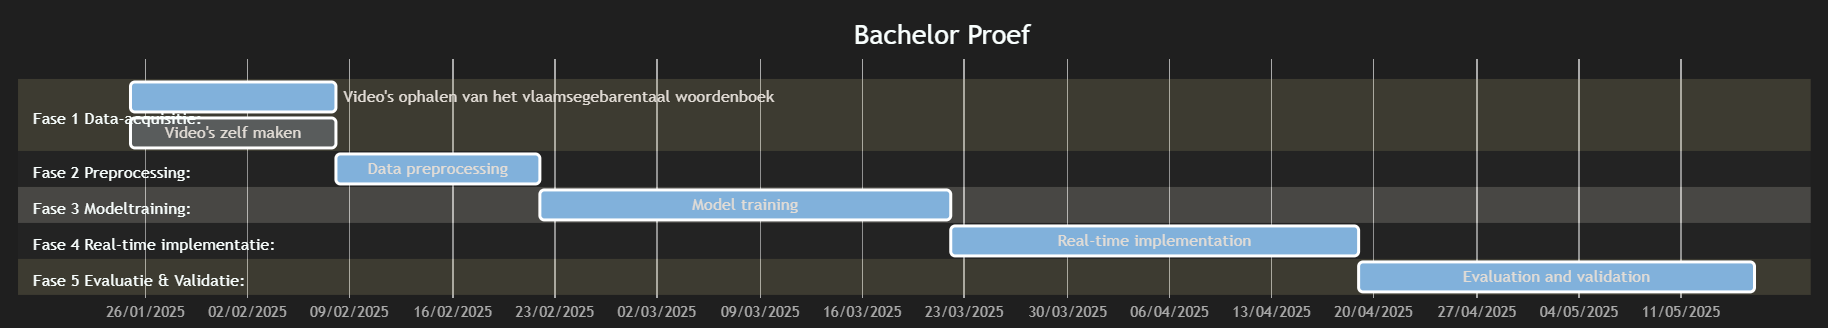
\includegraphics[width=0.5\textwidth]{../graphics/gantt_tijd.png}
  \caption{tijdlijn van het onderzoek}
  \label{fig:gantt_tijd}
\end{figure}
%---------- Verwachte resultaten ----------------------------------------------
\section{Verwacht resultaat, conclusie}%
\label{sec:verwachte_resultaten}
